\section{Amazon S3}
\label{sec:Amazon S3}

Amazon S3 (Simple Storage Service) is an online file storage web service offered by Amazon Web Services. Amazon S3 offers developers and IT teams a safe, durable and highly scalable storage solution.

Amazon S3 provides a convenient cost for object storage for a wide variety of use cases, such as cloud applications, content distribution, backup and archiving, disaster recovery and analysis of Big Data.

Amazon S3 offers different classes of storage designed for different use cases, including Amazon S3 Standard for generic data storage with frequent access, Amazon S3 Standard - Infrequent Access (Standard - IA) for data storage with less frequency access and Amazon Glacier for long-term storage.
Amazon S3 is reported to store more than 2 trillion objects as of April 2013.\cite{s3_stats} S3 uses include web hosting, image hosting, and storage for backup systems. 
Amazon S3 provides an API (Application programming interface) for third-party developers.

Today, there are different kinds of file managers for Amazon S3. 
Amazon provides an effective user interface that allows its users to browse, create and delete files and buckets.

\subsection{Amazon S3 Multipart Upload}
\label{subsec:amazon_S3_multipart_upload_initiation}


In the platform to upload videos Multipart upload API is used which enables to upload large objects quickly through the parallel upload of the n parts of the object.

Multipart uploading is a three-step process: initiate the upload, upload the object parts, and after all the parts have been uploaded, complete the multipart upload. Upon receiving the complete multipart upload request, Amazon S3 constructs the object from the uploaded parts, and you can then access the object just as you would any other object in your bucket.
You can access a list of all your in-progress multipart uploads or get a list of the parts that you have uploaded for a specific multipart upload.\cite{s3_multipart}


\begin{figure}[htb] %  figure placement: here, top, bottom
 \centering
 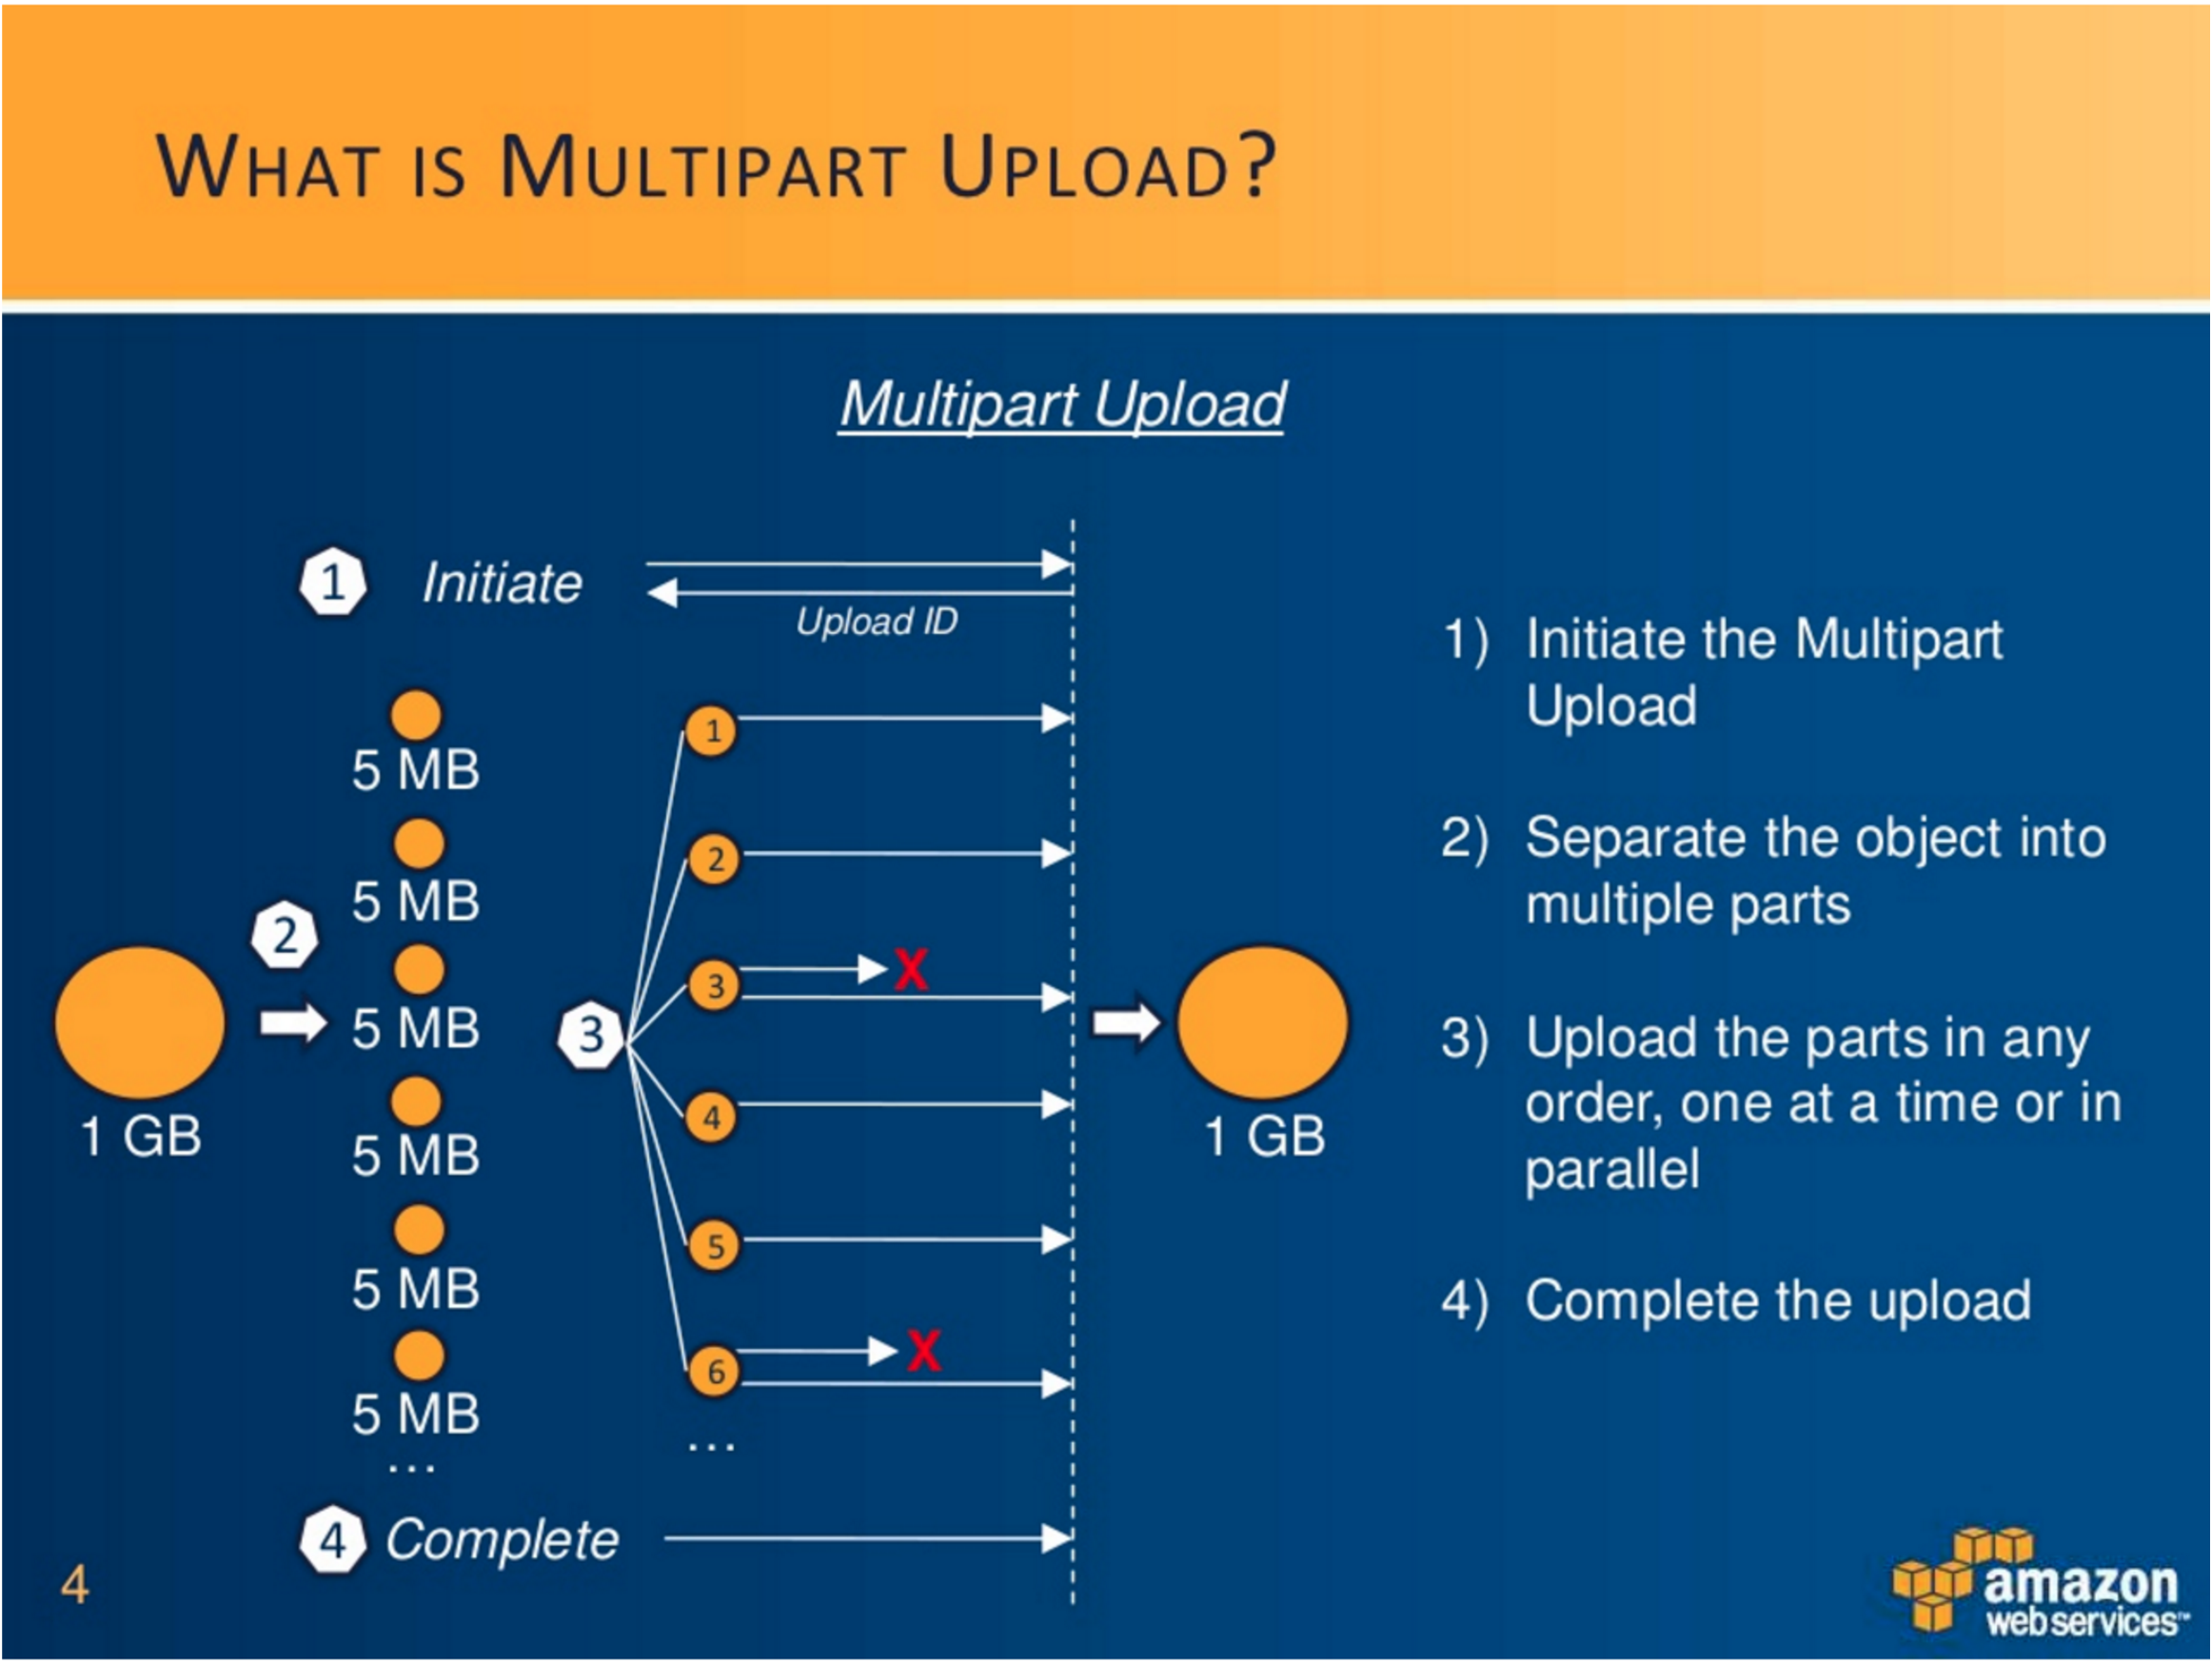
\includegraphics[width=1.0\linewidth]{images/chapter2/multipart_upload.png}\hfill
 \caption[Multi part Upload]{The MultiPart Upload}
 \label{fig:fourV}
\end{figure}

\subsection{Amazon S3 Multipart Upload Initiation}
\label{subsec:amazon_S3_multipart_upload_initiation}

When you send a request to initiate a multipart upload, Amazon S3 returns a response with an upload ID, which is a unique identifier for your multipart upload. You must include this upload ID whenever you upload parts, complete or abort an upload. If you want to provide any metadata describing the object being uploaded, you must provide it in the request to initiate multipart upload.


\subsection{Parts Upload}
\label{subsec:parts_upload}

When uploading a part, in addition to the upload ID, you must specify a part number. You can choose any part number between 1 and 10,000. A part number uniquely identifies a part and its position in the object you are uploading. If you upload a new part using the same part number as a previously uploaded part, this part is overwritten. Whenever you upload a part, Amazon S3 returns an ETag in its response header. For each part uploaded, you must record the part number and the ETag value. You need to include these values in the subsequent request to complete the multipart upload.
After you upload one or more parts, you must either complete or abort multipart upload in order to stop getting charged for storage of the uploaded parts. 


\subsection{Multipart Upload Completion (or Abort)}
\label{subsec:multipart_upload_completion}

When you complete a multipart upload, Amazon S3 creates an object by concatenating parts in ascending order based on the part number. If any object metadata was provided in the initiate multipart upload request, Amazon S3 associates that metadata with the object. After a successful complete request, the parts no longer exist. Your complete multipart upload request must include the upload ID and a list of both part numbers and corresponding ETag values. Amazon S3 response includes an ETag that uniquely identifies the combined object data. This ETag will not necessarily be an MD5 hash of the object data. You can optionally abort the multipart upload. After aborting a multipart upload, you cannot upload any part using that upload ID again. All storage that any parts from the aborted multipart upload consumed is then freed. If any part uploads were in-progress, they can still succeed or fail even after you aborted. To free all storage consumed by all parts, you must abort a multipart upload only after all part uploads have completed.

\begin{figure}[htb] %  figure placement: here, top, bottom
 \centering
 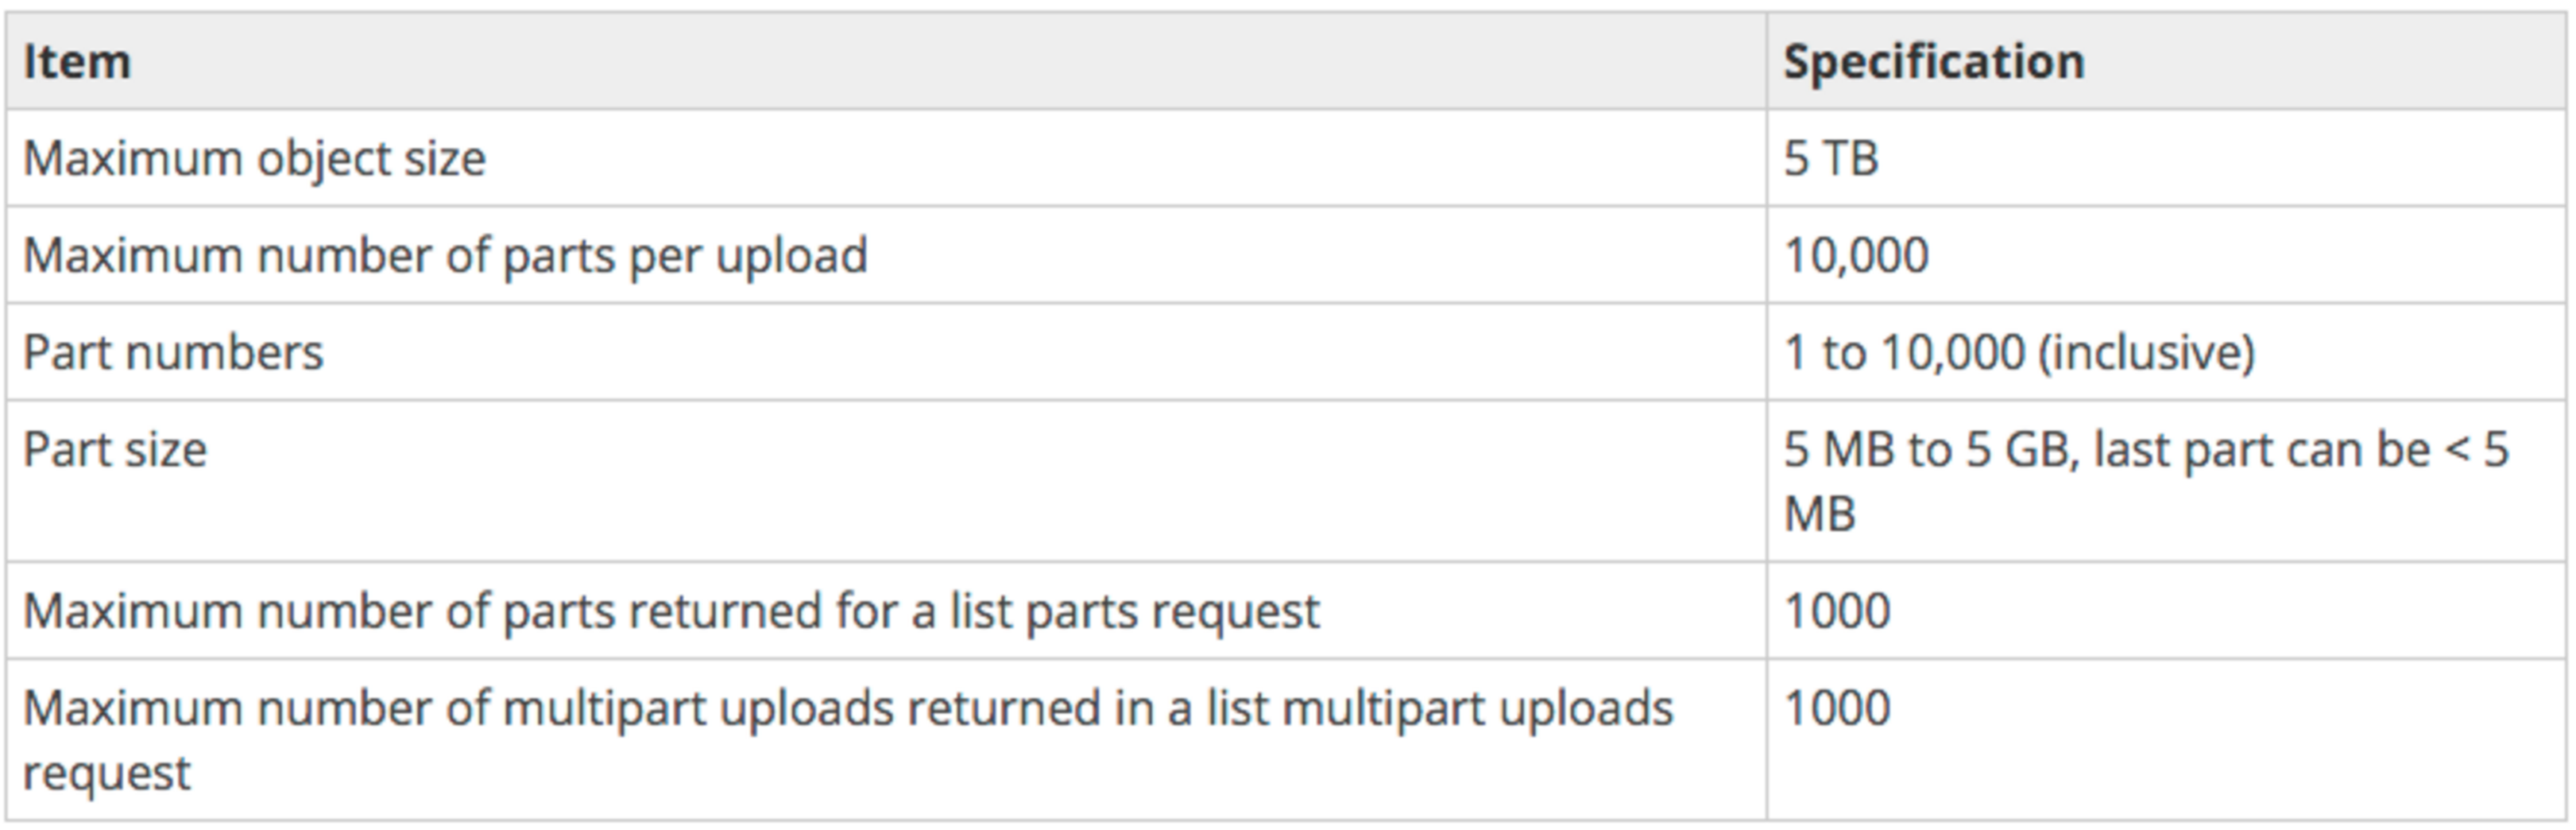
\includegraphics[width=1.0\linewidth]{images/chapter2/multi_part_info.png}\hfill
 \caption[Multi part Upload info]{The MultiPart Upload info}
 \label{fig:fourV}
\end{figure}
